\documentclass{beamer}

\usepackage{Vor2018glærur}

\title{Tölvunarfræði 2}
\subtitle{Vika 10}

\begin{document}

\begin{frame}
	\titlepage
\end{frame}

\section{Inngangur}

\begin{frame}{Úr viku 8}
	\begin{itemize}
		\item Vorum að skoða tvíleitartré \eng{binary search trees}
		\item Notuðum þau til að útfæra nafnatöflur \eng{symbol tables}
		\item Uppfletting og innsetning í nafnatöflu sem útfærð er með tvíleitartré er framkvæmanleg á logratíma
		      \begin{itemize}
			      \item \ldots sé tvíleitartréð í jafnvægi
		      \end{itemize}
		\item Skoðum leiðir til að tryggja logratíma
	\end{itemize}
\end{frame}

\imageslide{AlgsSlides/bst-shapes}

\section{2-3 tré}

\begin{frame}{2-3 tré}
	\begin{columns}
		\column{0.6\textwidth}
		\begin{itemize}
			\item Hugmynd - hvað ef við gætum geymt meira en einn lykil per hnút?
			\item Tvíleitartré hafa hingað til innihaldið nákvæmlega tvær vísanir, höfum verið með ``2-hnúta''
			      \begin{itemize}
				      \item Bætum nú við ``3-hnútum'' sem innihalda tvo lykla og þrjár vísanir
			      \end{itemize}
			\item Munum sjá að við getum notað þessa hugmynd til að tryggja jafnvægi - fjarlægð allra laufa frá rótinni er sú sama
		\end{itemize}
		\column{0.4\textwidth}
		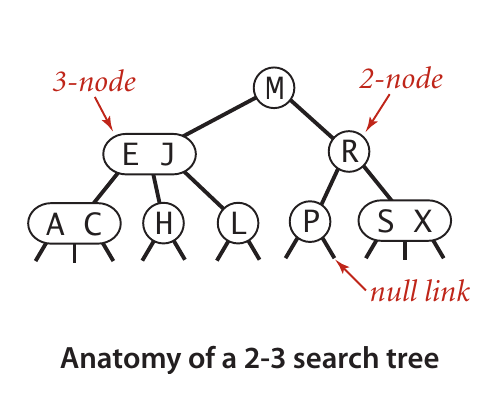
\includegraphics[width=\textwidth]{2-3-tree}

		Algorithms, 4th edition, bls. 424
	\end{columns}
\end{frame}

\begin{frame}{Endurkvæm skilgreining}
	\begin{itemize}
		\item 2-3 tré er tré sem er annaðhvort tómt eða:
		      \begin{itemize}
			      \item 2-hnútur með einn lykil og tvær vísanir. Vinstri vísun er í 2-3 tré með minni lykla og hægri vísun í 2-3 tré með stærri lykla.
			      \item 3-hnútur með tvo lykla og þrjár vísanir. Vinstri vísun í 2-3 tré með minni lykla, miðjuvísun í 2-3 tré með lykla sem liggja á milli vísa hnútsins og hægri vísun í 2-3 tré með stærri lykla.
		      \end{itemize}
	\end{itemize}
\end{frame}

\begin{frame}{Leit í 2-3 tré}
	\begin{center}
		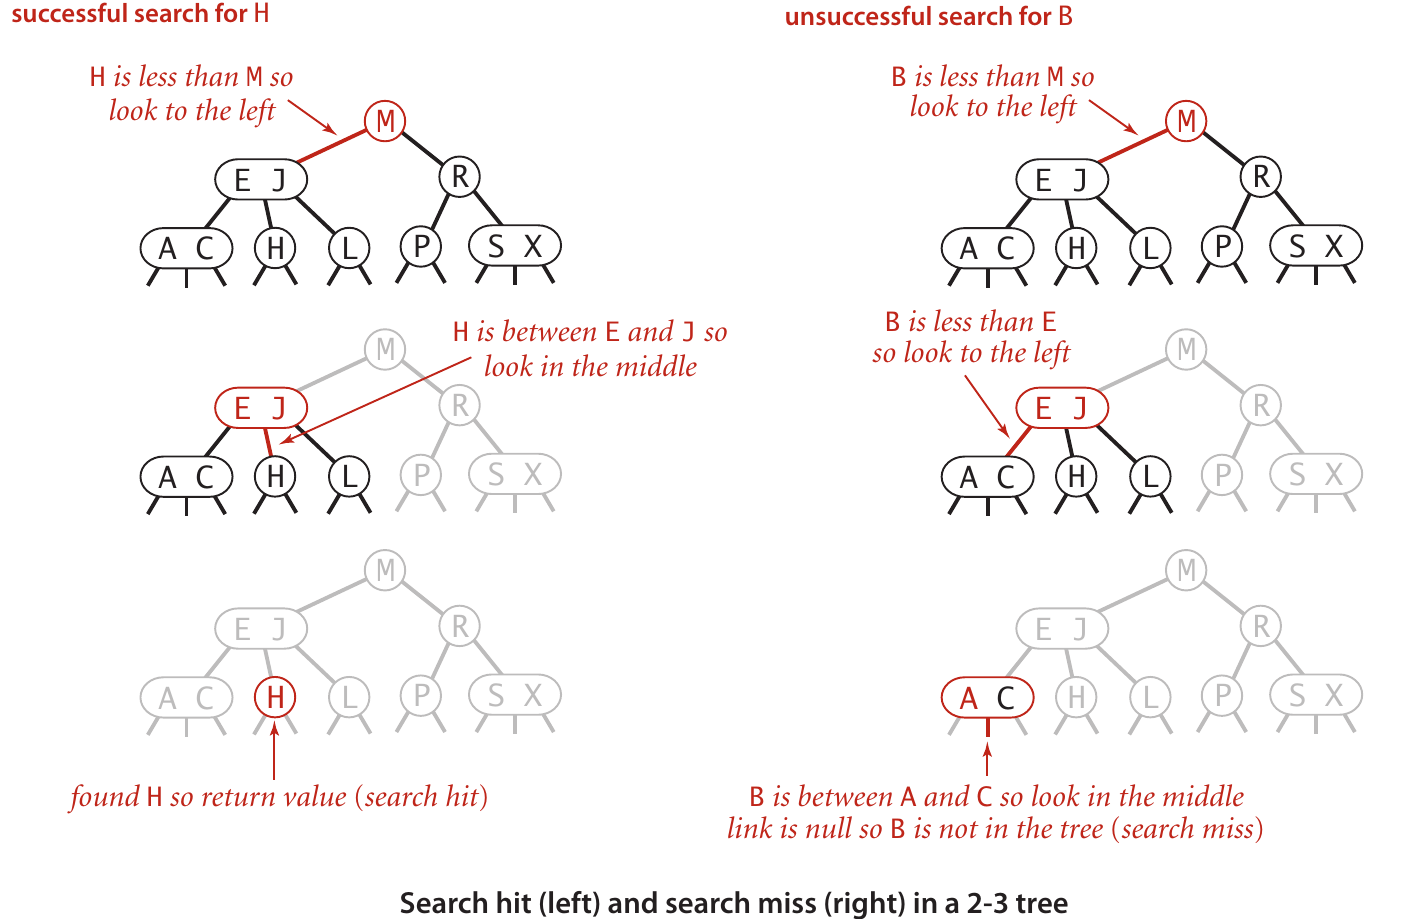
\includegraphics[width=0.9\textwidth]{2-3-tree-search}

		Algorithms, 4th edition, bls. 425
	\end{center}
\end{frame}

\imageslide{AlgsSlides/2-3-insertion-2-node}

\imageslide{AlgsSlides/2-3-insertion-3-node}

\begin{frame}{Athuganir}
	\begin{columns}
		\column{0.6\textwidth}
		\begin{itemize}
			\item Það að breyta 2-hnút í 3-hnút breytir ekki hæð trés
			\item Innsetning í 3-hnút veldur ekki hækkun á trénu nema hún valdi því að rótinni sé skipt upp
			\item Uppskipting á rótinni veldur \emph{samhverfri} hækkun
		\end{itemize}
		\column{0.4\textwidth}
		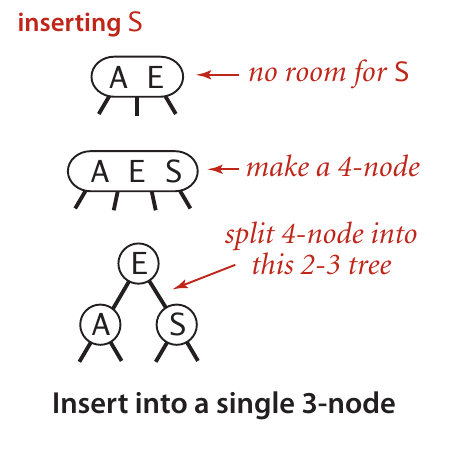
\includegraphics[width=\textwidth]{2-3-node-split}

		Algorithms, 4th edition, bls. 426
	\end{columns}
\end{frame}

\imageslide{AlgsSlides/2-3-insertion-local-transformation}

\imageslide{AlgsSlides/2-3-symmetric}

\imageslide{AlgsSlides/2-3-performance}

\begin{frame}{Vesen}
	\begin{itemize}
		\item Þægilegt er að hugsa um 2-3 tré og logratímatryggingin bregst ekki
		\item Hins vegar er beint-af-augum útfærslan bæði flókin og erfið
		      \begin{itemize}
			      \item Þyrftum margar gerðir af hnútum, hver einasta aðgerð krefst mikilla hreyfinga
			      \item Þó að innsetning fylgdi logratíma væri mikill fastur kostnaður
		      \end{itemize}
		\item Notum aðrar aðferðir til að útfæra innsýnina sem við fáum úr 2-3 trjám
	\end{itemize}
\end{frame}

\section{Rauðsvört tré}

\imageslide{AlgsSlides/red-black-introduction}

\imageslide{AlgsSlides/red-black-definition}

\imageslide{AlgsSlides/red-black-correspondence}

\imageslide{AlgsSlides/red-black-colors}

\imageslide{AlgsSlides/red-black-insert-overview}

\begin{frame}{Takmarkanir á yfirferð}
	\begin{columns}
		\column{0.30\textwidth}
		\begin{itemize}
			\item Snúningur á rauðsvörtum trjám er stórt viðfangsefni
			\item Farið í í kennslubók og í námskeiðinu Greining reiknirita
		\end{itemize}
		\column{0.30\textwidth}
		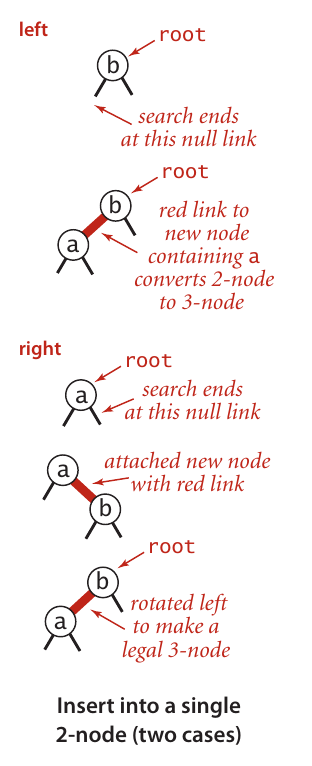
\includegraphics[width=\textwidth]{red-black-small-insert}
		\column{0.30\textwidth}
		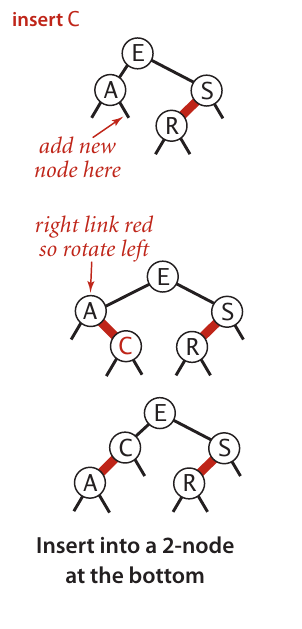
\includegraphics[width=\textwidth]{red-black-large-insert}
	\end{columns}
\end{frame}

\imageslide{AlgsSlides/red-black-balance}

\begin{frame}{Útfærslur á rauðsvörtum trjám}
	\begin{itemize}
		\item \texttt{RedBlackBST.java} í algs4 safninu
		\item \texttt{java.util.TreeMap}
		\item \texttt{std::map} í C++
		      \begin{itemize}
			      \item Sjá \texttt{mapexample.cpp}
		      \end{itemize}
	\end{itemize}
\end{frame}

\section{B-Tré}

\begin{frame}{B-tré}
	\begin{itemize}
		\item Hvað ef við myndum leyfa stærri hnúta en 3-hnúta?
		\item Gætum myndað tré þar sem hver hnútur inniheldur safn af gögnum
		      \begin{itemize}
			      \item Tréð verður ``lágt'' og ``breitt''
		      \end{itemize}
		\item Gagnlegt í kerfum þar sem við þurfum að sækja gögn út fyrir aðalminnið
	\end{itemize}
\end{frame}

\imageslide{AlgsSlides/b-tree-introduction}

\imageslide{AlgsSlides/b-tree-description}

\imageslide{AlgsSlides/b-tree-search}

\imageslide{AlgsSlides/b-tree-insertion}

\imageslide{AlgsSlides/b-tree-performance}

\section{Hakkaföll}

\begin{frame}{Einfaldasta uppflettingin}
	\begin{columns}
		\column{0.7\textwidth}
		\begin{itemize}
			\item Athugum: Væru lyklar alltaf heiltölur gætum við notað fylki til að útfæra skilvirka nafnatöflu
			\item Búum til fylki úr gildunum, svo að tilsvarandi gildi lykilsins $i$ sé í sætisnúmeri $i$
			\item Þyrftum stórt fylki, en uppfletting væri framkvæmanleg á föstum tíma
			      \begin{itemize}
				      \item Dæmi um ``space-time tradeoff''
			      \end{itemize}
		\end{itemize}
		\column{0.3\textwidth}
		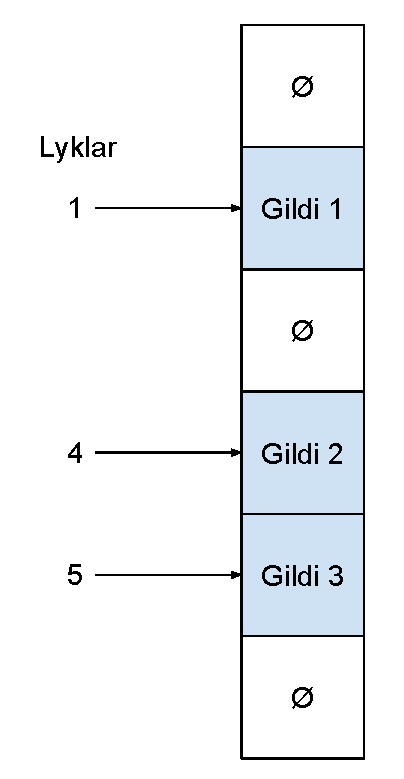
\includegraphics[width=\textwidth]{array-st}
	\end{columns}
\end{frame}

\begin{frame}{Hakkaföll}
	\begin{columns}
		\column{0.5\textwidth}
		\begin{itemize}
			\item Vandamál 1: Oft eru lyklarnir ekki heiltölur
			\item Vandamál 2: Heiltölur á stóru bili krefjast risastórs fylkis
			\item Lausn: Skrifum hakkafall \eng{hash function} sem varpar lyklunum okkar í heiltölur á ákveðnu bili
		\end{itemize}
		\column{0.5\textwidth}
		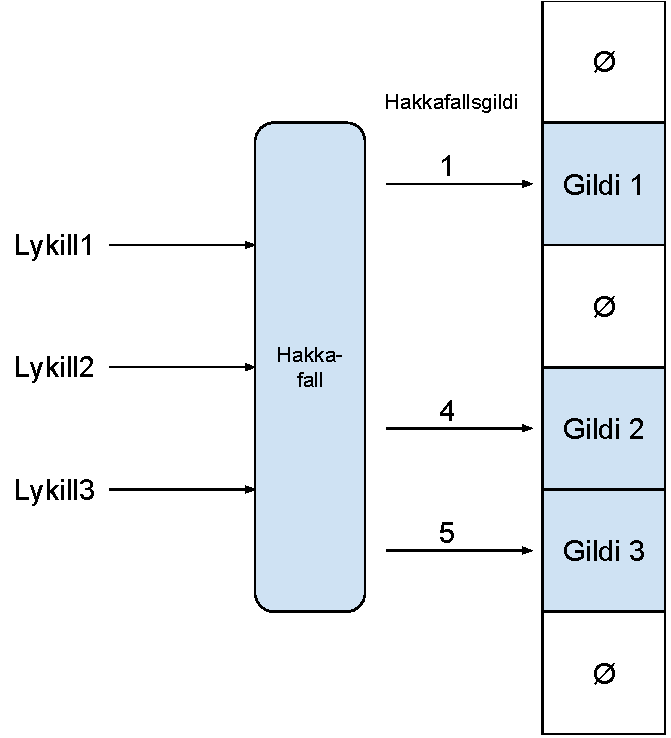
\includegraphics[width=\textwidth]{hash-function}
	\end{columns}
\end{frame}

\begin{frame}{Hakkatöflur}
	\begin{itemize}
		\item Útfærsla á hakkatöflu \eng{hash table} felur tvennt í sér
		      \begin{itemize}
			      \item Hakkafall \eng{hash function} sem varpar $n$ lyklum yfir í sætisnúmer $m$ staka fylkis
			      \item Leið til að ákveða hvað gerist þegar hakkafallið varpar tveim lyklum í sama sætisnúmer \eng{collision resolution process}
		      \end{itemize}
		\item Hvort tveggja tekur fastan ``heildarmeðaltíma'' þegar vel tekst til
	\end{itemize}
\end{frame}

\imageslide{AlgsSlides/java-hashcode}

\imageslide{AlgsSlides/java-simple-hashcodes}

\imageslide{AlgsSlides/java-string-hashcode}

\begin{frame}[fragile]{Lokaskref}
	\begin{itemize}
		\item Hakkatöfluútfærslur treysta á að hakkafallsgildin séu jafndreifð
		      \begin{itemize}
			      \item Ef við förum langt frá þessari forsendu munum við þurfa endurtekið að fást við árekstra
		      \end{itemize}
        \item Við þurfum líka að breyta skilagildi \texttt{hashCode()} í tölu frá $0$ upp í $m-1$ (þar sem $m$ er stærð fylkisins okkar)
        \item Í algs4 er formerkisbitanum hent og deilingarafgangur reiknaður:
    \end{itemize}
		      \begin{minted}[frame=lines]{java}
private int hash(Key x){ 
    return (x.hashCode() & 0x7fffffff) % M; 
}
\end{minted}
	
\end{frame}

\section{Hakkatöfluútfærslur}

\imageslide{AlgsSlides/hash-collisions}

\imageslide{AlgsSlides/hash-separate-chaining}

\imageslide{AlgsSlides/hash-separate-chaining-java}

\imageslide{AlgsSlides/hash-separate-chaining-analysis}

\imageslide{AlgsSlides/hash-separate-chaining-resizing}

\imageslide{AlgsSlides/hash-linear-probing}

\imageslide{AlgsSlides/hash-linear-probing-java-get}

\imageslide{AlgsSlides/hash-linear-probing-java-put}

\imageslide{AlgsSlides/hash-linear-probing-analysis}

\imageslide{AlgsSlides/symbol-table-summary}

\begin{frame}{Þessi glærupakki}

	Kóða fyrir algs4 reiknirit má finna á \url{http://algs4.cs.princeton.edu/code/}.

	Glærur með gráan bakgrunn má finna á \url{https://algs4.cs.princeton.edu/lectures/}.

	Sýniforrit má finna á \href{https://github.com/Ernir/kennsluefni/tree/master/T2/Code/w10}{Github}.

\end{frame}

\begin{frame}{Næst}
	Net (Kaflar 4.1 og 4.2)
\end{frame}

\end{document}
